\section{Introdução}

\begin{frame}[fragile]{Histórico}

    \begin{itemize}
        \item Os primeiros compiladores surgiram na década de 50
        %\pause

        \item Não há registros preciso de qual foi o primeiro compilador
        %\pause

        \item Os primeiros compiladores lidavam com a tradução de fórmulas aritméticas (FORTRAN -- \textit{Formula Translator})
        %\pause

        \item Os compiladores eram considerados programas difíceis de se escrever
        %\pause

        \item O primeiro compilador Fortran levou 18 homens-ano para ser escrito (1 homen-ano $\approx$ 2.080 horas)
        %\pause

        \item Embora continue não sendo uma tarefa não trivial, a escrita de compiladores se beneficiou dos avanços da área desde então
    \end{itemize}

\end{frame}


\begin{frame}[fragile]{Definição}

    \begin{block}{Definição de compilador (informal)}
        Um compilador é um programa que lê um programa escrito em uma linguagem (linguagem fonte) e o traduz para uma outra linguagem (linguagem alvo).
    \end{block}

    %\pause

    \vspace{0.2in}

    \begin{center}
    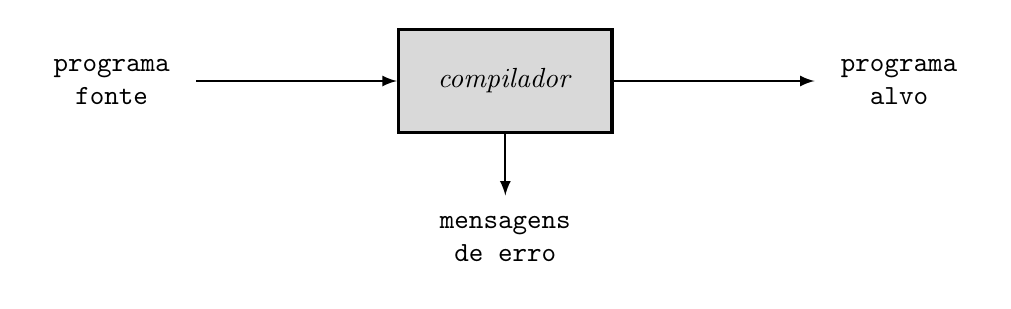
\begin{tikzpicture}
        \node (A) at (0, 0) { \begin{tabular}{c}\texttt{programa}\\ \texttt{fonte}\end{tabular} };
        \node[draw,very thick,fill=gray!30,inner sep=0.5cm] (B) at (5, 0) { \textit{compilador} };
        \node (C) at (10, 0) { \begin{tabular}{c}\texttt{programa}\\ \texttt{alvo}\end{tabular} };
        \node (D) at (5, -2) { \begin{tabular}{c}\texttt{mensagens}\\ \texttt{de erro}\end{tabular} };

        \draw[-latex,thick] (A) to (B);
        \draw[-latex,thick] (B) to (C);
        \draw[-latex,thick] (B) to (D);
    \end{tikzpicture}
    \end{center}

\end{frame}

\begin{frame}[fragile]{Características dos compiladores}

    \begin{itemize}
        \item O processo de compilação deve identificar e relatar possíveis erros no programa fonte
        %\pause

        \item Em geral, as linguagens fonte são linguagens de programação tradicionais (C/C++, Java, Python, etc)
        %\pause

        \item As linguagens alvo podem ser tanto linguagens tradicionais quanto linguagens de máquina
        %\pause

        \item Os compiladores podem ser classificados de diversas formas, dependendo de seu objetivo ou como foi construído (de uma passagem, múltiplas passagens,
            depuradores, etc)
    \end{itemize}

\end{frame}

\begin{frame}[fragile]{Criação do programa executável}

    \begin{itemize}
        \item Além do compilador, outros programas podem ser usados na criação do programa executável
        %\pause

        \item Antes de ser passado para o compilador, o programa alvo pode ser pré-processado (por exemplo, o pré-processador da linguagem C processa as
            diretivas como \mintinline{cpp}{#include} e \mintinline{c}{#define})
        %\pause

        \item Após a compilação, o programa alvo pode demandar processamento adicional para a construção do executável (novamente no caso da linguagem C, temos
            o montador e o \textit{linkeditor})

    \end{itemize}

\end{frame}

\begin{frame}[fragile]{Exemplo de fluxo de geração de um programa executável}

    \begin{figure}
        \centering

        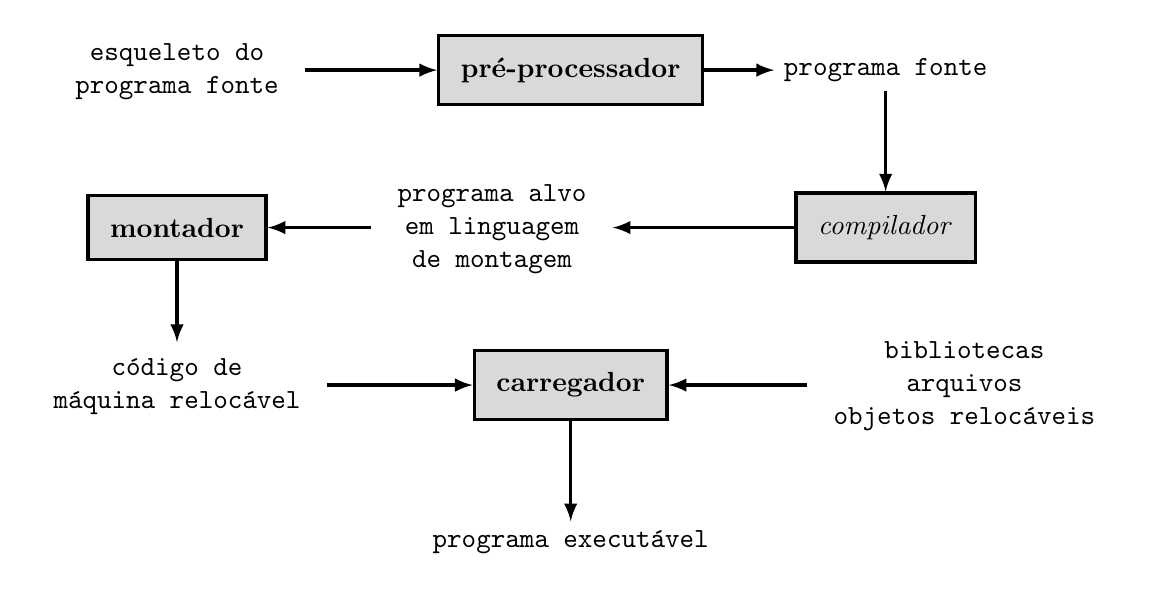
\begin{tikzpicture} 
            \node (A) at (-1, 6) { \begin{tabular}{c}\texttt{esqueleto do}\\ \texttt{programa fonte}\end{tabular} };
            \node[draw,very thick, fill=gray!30, inner sep=8pt] (B) at (4, 6) { \textbf{pré-processador} };
            \node (C) at (8, 6) { \texttt{programa fonte} };
            \node[draw,very thick, fill=gray!30, inner sep=8pt] (D) at (8, 4) { \textit{compilador} };
            \node (E) at (3, 4) { \begin{tabular}{c}\texttt{programa alvo}\\ \texttt{em linguagem}\\ \texttt{de montagem}\end{tabular} };
            \node[draw,very thick, fill=gray!30, inner sep=8pt] (F) at (-1, 4) { \textbf{montador} };
            \node (G) at (-1, 2) { \begin{tabular}{c}\texttt{código de}\\ \texttt{máquina relocável}\end{tabular} };
            \node[draw,very thick, fill=gray!30, inner sep=8pt] (H) at (4, 2) { \textbf{carregador} };
            \node (I) at (9, 2) { \begin{tabular}{c}\texttt{bibliotecas}\\ \texttt{arquivos}\\ \texttt{objetos relocáveis}\end{tabular} };
            \node (J) at (4, 0) { \texttt{programa executável} };

            \draw[very thick,-latex] (A) to (B);
            \draw[very thick,-latex] (B) to (C);
            \draw[very thick,-latex] (C) to (D);
            \draw[very thick,-latex] (D) to (E);
            \draw[very thick,-latex] (E) to (F);
            \draw[very thick,-latex] (F) to (G);
            \draw[very thick,-latex] (G) to (H);
            \draw[very thick,-latex] (I) to (H);
            \draw[very thick,-latex] (H) to (J);
        \end{tikzpicture} 
    \end{figure}

\end{frame}
